\thispagestyle{plain}
	\AddToShipoutPictureBG*{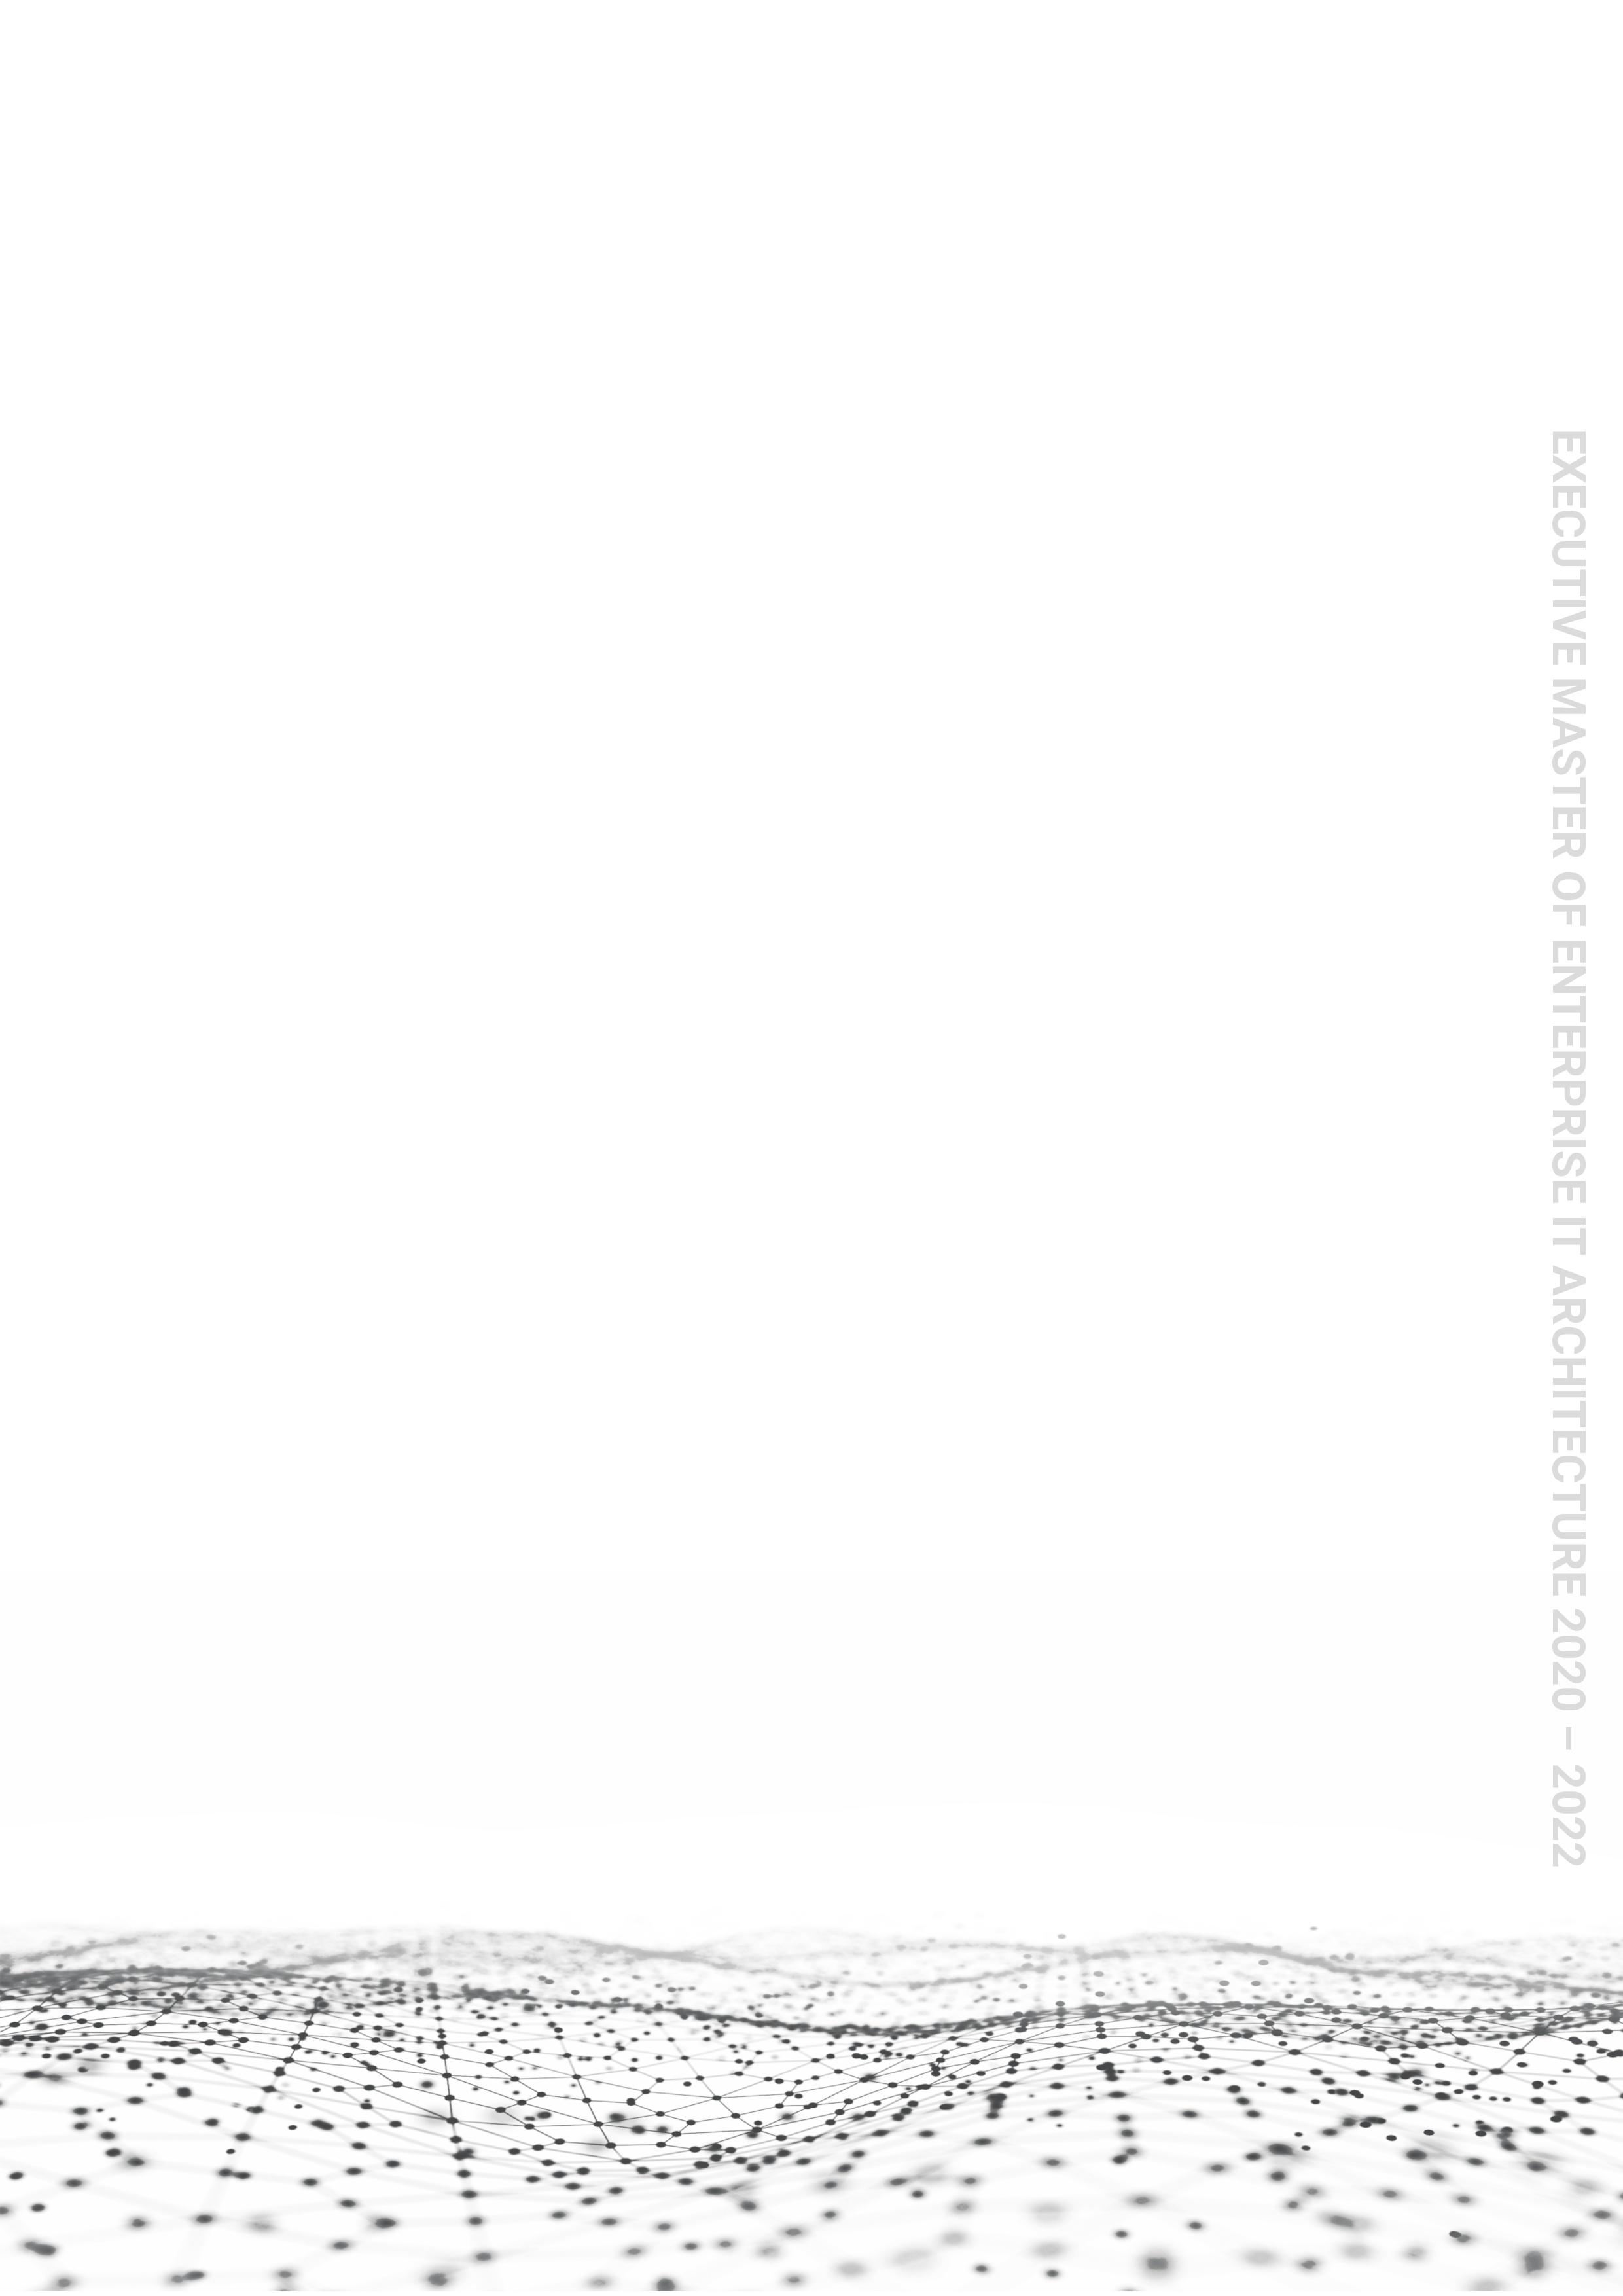
\includegraphics[width=\paperwidth,height=\paperheight]{background}}
\begin{center}
	\Large
	\textbf{Errata for submission ID 15932}

	\vspace{0.3cm}
	\textbf{Towards an Antifragile Public Sector}
	
	\vspace{0.3cm}
	\large
	Introducing antifragility in the Dutch Public Sector with Enterprise Architecture

	\vspace{0.3cm}
	\textbf{René Bliekendaal}
		
	\vspace{0.4cm}
\end{center}

\begin{table}[H]
	\centering
	\begin{tabular}{p{0.07\textwidth}p{0.4\linewidth}p{0.4\linewidth}}
		\toprule
		\textbf{Page} & \textbf{Original} & \textbf{Proposed change} \\
		\midrule
		Exec. Sum. & ... that are responsive and adaptive. & ... that are responsive and adaptive. \textbf{In his essay, van der Steen (2018, p. 79) tossed the concept antifragile from Taleb (2012) as a possible direction to create an adaptive government.} \\%
		1 & ... unpredictable environment (Nijssen et al., 2018, pp. 1–2). & ... unpredictable environment (Nijssen et al., 2018, pp. 1–2).  \textbf{In his essay, van der Steen (2018, p. 79) tossed the concept antifragile from Taleb (2012) as a possible direction to create an adaptive government.} \\%
		16 & Definition of Graves (2009, p. 5): Enterprise Architecture is the organising logic for business processes and IT infrastructure, reflecting its operating model’s integration and standardisation requirements. It provides a long term view of a company’s processes, systems and technologies so that individuals can build capabilities and not just fulfil immediate needs. & Definition of Graves (2009, \textbf{pp. 4--5): Enterprise Architecture is a discipline through which an Enterprise can identify, develop and manage its knowledge of its purpose, its structure and itself. Enterprise Architecture will also assist in managing changes imposed on the organisation by the market, by regulations, or -- at an operations level -- by system failures, environmental incidents or customer complaints.}  \\%
		\bottomrule
	\end{tabular}%
\end{table}%


